\documentclass[a4paper,10pt,DIV10,openright,openbib]{scrreprt}
\usepackage[utf8]{inputenc}
\usepackage[T1]{fontenc}
\usepackage[english]{babel}
\usepackage[fixlanguage]{babelbib}
\selectbiblanguage{english}
\usepackage{float}
\usepackage{scrpage2}   %KOMA PG Settings
\usepackage{tocloft}    %ToC Control
\usepackage{graphicx}   %Better graphics
\usepackage{wrapfig}    %Better wrap text around figures
\usepackage{array}      %Array Evironments (Matrices,etc)
\usepackage{tabularx}   %Better Tables
\usepackage{tikz}       %Tikz
\usepackage{pdfpages}   %Append PDF
\usepackage[english]{varioref}  %Intelligent page refs
\usepackage{makeidx}    %Index
\usepackage{listings}   %Better Listings
\usepackage{textcomp}   %Unicode Block
\usepackage{hyperref}   %Clickable links in .pdf
\usepackage{caption}    %Custom Caps in Floats
\usepackage{rotating}
\usepackage{mathtools}  %fancy arrows
\usepackage{amsmath}
\usepackage{booktabs}
\usepackage{titling}
\setcounter{secnumdepth}{3}
\setcounter{tocdepth}{1}
\usepackage[stable]{footmisc}
\setlength{\textheight}{1.1\textheight} %BREAKS FOOTER?
% \usepackage{showframe} %DEBUG
\usepackage{pgf-pie}


% Bibliography no pagebreak:
\let\oldbibliography\bibliography% Store \bibliography in \oldbibliography
\renewcommand{\bibliography}[1]{{%
  \let\chapter\section% Copy \section over \chapter
  \oldbibliography{#1}}}% Old \bibliography


\RedeclareSectionCommand[
  beforeskip=-1.0\baselineskip,
  afterskip=-1\baselineskip]{subsection}
\RedeclareSectionCommand[
  beforeskip=-.75\baselineskip,
  afterskip=-1\baselineskip]{subsubsection}
\RedeclareSectionCommand[
  beforeskip=-2sp,
  afterskip=2\baselineskip]{chapter}
\makeindex
    \renewcommand{\abstractname}{System Background}
\usepackage{listings}
\usepackage{color}
 
\definecolor{codegreen}{rgb}{0,0.6,0}
\definecolor{codegray}{rgb}{0.5,0.5,0.5}
\definecolor{codepurple}{rgb}{0.58,0,0.82}
\definecolor{backcolour}{rgb}{0.95,0.95,0.92}
 
\lstdefinestyle{mystyle}{
    backgroundcolor=\color{backcolour},   
    commentstyle=\color{codegreen},
    keywordstyle=\color{magenta},
    numberstyle=\tiny\color{codegray},
    stringstyle=\color{codepurple},
    basicstyle=\footnotesize,
    breakatwhitespace=false,         
    breaklines=true,                 
    captionpos=b,                    
    keepspaces=true,                 
    numbers=left,                    
    numbersep=5pt,                  
    showspaces=false,                
    showstringspaces=false,
    showtabs=false,                  
    tabsize=2
}
 
\lstset{style=mystyle}

\begin{document}


%----------------------------
% Title
% ----------------------------
%titlepage
\thispagestyle{empty}
\begin{center}
\begin{minipage}{0.75\linewidth}
    \centering
%University logo
    
\includegraphics[width=120px,height=120px]{avatar-logo-blueonwhite.png} \\[0.3\baselineskip]
    \vspace{2cm}
%Thesis title
    {\uppercase{\Large System Design Project: \\ Project Plan\par}}
    \vspace{3cm}
%Author's name
    {\large Authors: \\
      Stefani Genkova   - \textit{s1437453} \\
      Tizzy MacGregor   - \textit{s1508959} \\
      Glen Merry        - \textit{s1531807} \\
      Alexander Pietz   - \textit{s1529373} \\
      Jasper Snel       - \textit{s1452790} \\
      Philip Van Biljon - \textit{s1545259} \\
      Boyan Yotov       - \textit{s1509922} \\
    \par} 
    \vspace{3cm}
%Degree
    {\Large DispensED - Group 17 \par}
    \vspace{3cm}
%Date
    {\small Last Update: \today}
\end{minipage}
\end{center}
\clearpage
%----------------------------
% /Title
%----------------------------
\newpage

\tableofcontents
% \listoffigures

\pagestyle{plain}
%\chapter{System Background}
%\section{System Description}

\section{Purpose of this Document}
This document is prepared as part of the project for the System Design Project course
at the University of Edinburgh. This project plan will highlight the goals we
have set as a team as well as how we will achieve them - Including a breakdown
of our resources and overview of our organisational structure.
\vspace{2cm}
{\let\clearpage\relax  \chapter{Goals}}
% 3 marks ~1.5 pages
% The goal description should give an overview of the user problem and the robot
% task solution you propose. This could be in the form of a user story. If
% appropriate, include reference to existing systems that you are taking as
% inspiration, or published evidence for the user need that you plan to address.
% You should then breakdown the overall problem into the main technical
% subgoals, i.e., what you need to accomplish to get to the desired final
% result. For each subgoal you should provide an explicit milestone that states
% what you should have achieved, by what date, and what evidence you will
% present to show you have achieved it (e.g. a demonstration of the feature to
% your client).

There is a large shortage of nursing staff across the UK. The NHS alone reported
that nurses account for 38\% of overall vacancies\footnote{http://digital.nhs.uk/catalogue/PUB30033}.
Care home staff, specifically, spend about 40-50\% of their time with drug
related activities. Administration errors occur 8.4\% of the time \cite{CHUMS},
meaning if a patient receives medication three times a day, there is a 1 in 4
chance that an error occurs.\\
DispensED is aiming to develop a solution to the problems created by manual drug
administration by creating a robot to do the bulk of the work. Our product will
move around care homes to different residents' homes. The residents can then
scan their identification and the appropriate drugs and vitamins will be
dispensed. The system will also have a wide range of administrative functions
available to staff, such as setting alerts on low stock levels or non-admittance of drugs.

\section{Technical Subgoals}
\subsection{Communication}
The robot needs to communicate with a DICE machine that will support vision and
connection to the back-end.
\subsection{Movement}
The robot needs to be able to move along the facility it is being deployed in.
The navigation will happen along predefined routes using marks on the floor.
Additional care must be taken in regards to possible collisions as the robot
will operate in a generally dynamic environment. 
\subsection{Vision}
Several vision systems are needed in order for the robot to accomplish its objective:
\subsubsection{Orientation}
The robot must be able to recognise and process the markings on the floor that
are used for navigation. Additionally, the system must know where the rooms are
it is trying to service - separate floor markings or an alternative kind of
internal representation of the environment may be used for this.
\subsubsection{Barcode Scanning}
Medication is dispensed to the patient after they have authorised themselves.
The main form of authorisation will be bar codes (these could be affixed to the
patients' wristbands). The system must be able to read the barcodes

\subsection{Dispensing of Medication}
The robot will support giving out medication in two different ways:
\subsubsection{Pre Packed Sets of Medication} Most care homes get pharmaceutical drugs come
pre-packed from the pharmacy, sorted by patient. In this case, the robot must
give out the container with the pre-packaged drugs to the correct patient. There
needs to be support to store drugs for several different people that may not
collect their drugs in order.
\subsubsection{Single Pills (Vitamins)} For pills that do not come pre-packed
(such as vitamins), a different kind of dispenser is needed. This dispenser must
be able to give out single pills, one at a time.

\subsection{Back-end}
The back-end will offer a range of configuration as well as storing the patient
database. Configured alerts will be sent out from the back-end, too.
\subsubsection{Database} The Database will store patient information, including
which room they reside in and their daily medication preferences. These
preferences include:
\begin{itemize}
  \item Patient information
  \item Type of medication needed (pre-packaged and/or loose?)
  \item Deadline for drug admission (to send out alerts)
\end{itemize}
\subsubsection{User Interface} There will be a user interface to serve as the
front-end to the aforementioned configuration.

\\ TODO : ADD MILESTONES HERE \newpage

{\let\clearpage\relax \chapter{Resource Allocation}}
% 3 marks for time planning ~1.5 pages
% 3 marks for identification of dependencies and risks ~1.5 pages
% The plan should explain how you will deploy your resources - 200 hours per
% group member over the semester - to achieve your goals. Note you should take
% into account time required by scheduled sessions (guest lectures, demo days,
% final presentations) and time used in planning and presenting (group meetings,
% report writing etc.), as well as time for building the system. You should also
% note the resources you have in terms of skills, equipment, etc. You must
% include a Gantt chart, which should clearly identify any dependencies between
% tasks. You may find it useful to make a revised version of your plan/gantt
% chart at key points in the project, in discussion with your client. The report
% should also contain an assessment of the risks that you anticipate for the
% project, and contingency planning that you have done to guard against them.

% Guest lectures: 8hrs 
% Demos and Pitches: 8hrs
% Planning and Presenting: 30hrs
% Development work: 150hrs
% Miscellaneous: 4hrs
\begin{figure}[h]
  \centring
  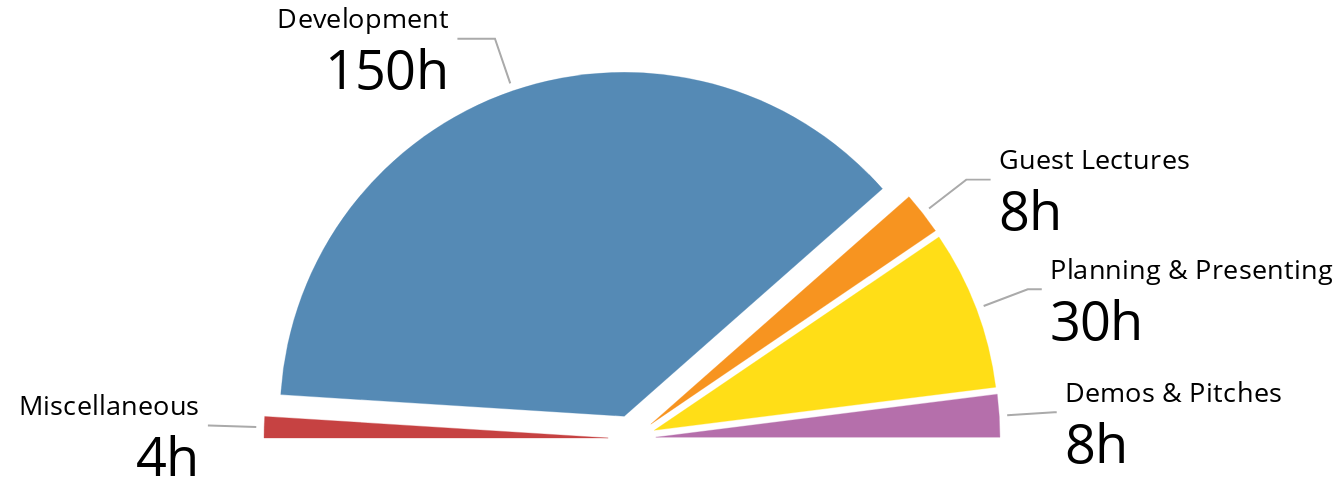
\includegraphics[width=\textwidth]{pie.png}
  \caption{Planned Time Deployment}
\end{figure}

\section{Risks and Contingency Planning}
The most apparent risk that would hinder project progress is absence of team members. 
As mentioned above, %mention this :D
we split our team into different sub-teams. Every sub team has multiple members and 
the project management ensures that no one team member has knowledge that no other 
team member possesses. This way, the impact of any one team member being ill or 
otherwise unable to work is minimised. Other risks arise from 



{\let\clearpage\relax \chapter{Organisational Structure}}
% 3 marks ~1.5 pages
% Finally, how you organise yourselves as a group and plan your work will be key
% to your success within the System Design project. You should detail the
% approach that you have taken to group organisation (e.g. specific roles of
% group members), meetings, communication, code-sharing, task allocation, and
% progress tracking.
\section{Team Structure}
The team structure follows loosely a Functional Matrix structure. Alexander was
assigned as key contact and team manager. As previously mentioned, we split our
team up into multiple sub-teams working towards the sub-goals of their area. The
bold person is the ``owner'' of the groups work, meaning they are the first
point of contact.
\begin{table}[]
\centering
\begin{tabular}{@{}llll@{}}
\toprule
Medication Dispensing & \begin{tabular}[c]{@{}l@{}}Software\\ Back \& Front End\end{tabular} & \begin{tabular}[c]{@{}l@{}}Movement \\ (physical)\end{tabular} & Vision          \\ \midrule
\textbf{Glen}         & \textbf{Alex}                                                        & \textbf{Philip}                                                & \textbf{Jasper} \\
Tizzy                 & Bobby                                                                & Jasper                                                         & Stefani         \\
Philip                & Glen                                                                 & Bobby                                                          &                 \\
Stefani               & Tizzy                                                                & Alex                                                           &                 \\ \bottomrule
\end{tabular}
\caption{Sub Teams}
\end{table}

\section{Meetings}
Every morning an informal catch-up is held so that everyone is able to be up to
date with the current state of the system. These catch-ups usually just include
any progress from the previous day as well as potential new issues / roadblocks
that may have emerged.\\
The whole team meets with our mentor during a one hour fixed meeting slot on
Thursdays at noon - everyone is expected to attend these meetings.
Additional meetings follow a drop-in approach and are conducted as needed.


\section{Communication and Tools}
The main vector of communication is the team slack - we use Notion as platform for notes,
drafts and project management. Specific tasks are allocated via trello-like boards in
the To-Do section on notion. We decided to use Notion instead of Trello as it
offers additional functionality. The way we manage both task allocation and
progress tracking follows SCRUMBAN management system, a mix between SCRUM
and KANBAN. This system picks out the most useful agile parts from KANBAN while
maintaining clearly defined roles - We hope this will aid our team with more
steady progress whilst not locking ourselves into an engineering process that
requires planning very far ahead. \\
A private GitHub repository for code version control has been set
up for the project. We have used GitHub as it was the most accessible since
everyone already had an account.\\
\begin{table}[h]
\centering
\caption{Tool Overview}
\begin{tabular}{@{}lll@{}}
\toprule
Tool   & Purpose                                   & Link     \\ \midrule
Slack  & Main Communications HUB, Chat             & \url{https://sdpgroup17.slack.com/} \\
Notion & Meeting Notes, Drafts, Project Management & \url{https://www.notion.so/dispensed/} \\
GitHub & Code Version Control                      & \url{https://github.com/xMythycle/DispensED/} \\ \bottomrule
\end{tabular}
\end{table}


%\bibliographystyle{alpha}
\bibliographystyle{alphadin}
\bibliography{Bibl}
%\begingroup
%\printindex 
%\endgroup

   
\end{document}